\chapter{Teoretický úvod}

V~této kapitole přiblížíme některé pojmy a teorie, které jsou v~práci využity.

\section{Zrakové vyhledávání}

V~úloze zrakového vyhledávání je úkolem najít ve scéně stimul s~určitými
vlastnostmi. Tyto scény mohou být jednoduché, jako například několik černých
úseček na bílém pozadí, kdy je úkolem najít úsečku, která má určitý směr. Pro
konkrétní příklad úlohy zrakového vyhledávání viz obrázek \ref{obr:tecka}.
I~takto jednoduché úlohy ale mají mnoho společného se zrakovým vyhledáváním tak,
jak ho provádíme v~běžném životě \citep{VisualSearch}. Mohou ale také být velmi
komplikované a těžko popsatelné, jako například hledání muže v~pruhovaném
oblečení, jaké známe z~populární úlohy \uv{Kde je Valda?}.  

\begin{figure}[h!]
 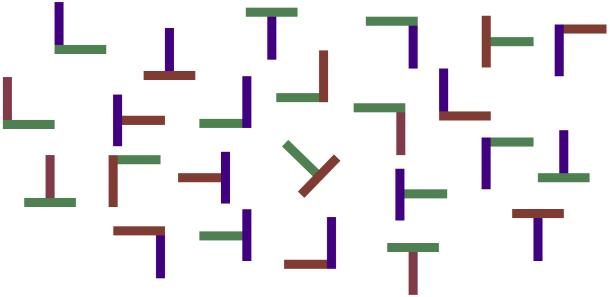
\includegraphics[width=.9\linewidth]{img/tecka}
  \centering
\caption{Příklad jednoduché úlohy zrakového vyhledávání. Úkolem pozorovatele je zde najít čtyři fialovo-zelená písmena T.} 
\label{obr:tecka}
\end{figure}

Předchozí výzkum ukázal, že lidští
pozorovatelé v~této úloze využívají krátkých pohledů a rychlých pohybů očí \citep{Holmquist}.
Jednomu takovému krátkému pohledu budeme říkat \emph{fixace}. Rychlému očnímu pohybu
se říká \emph{sakáda} \citep{sakady}.

Při vyhledávání nás ve skutečnosti zajímá, ke kterým místům pozorovatel obrací
svou pozornost. To však výrazně souvisí s~tím, kam se kouká \citep{Attention}.


\section{Úvod do teorie detekce signálu}

Jeden z~dílčích problémů úlohy zrakového vyhledávání je rozlišení hledaného
objektu a pozadí. K~popisu řešení tohoto problému se nám bude hodit
terminologie teorie detekce signálu, která se právě touto problematikou
zaobírá.

V~řeči této teorie budeme hledanému objektu říkat {\it signál},
rušivým elementům ve scéně se říká {\it šum}. Problém rozlišení hledaného
objektu a pozadí se tedy v~řeči teorie detekce signálu formulují jako dotaz,
zda se v~dané lokaci signál nachází, či nenachází. Tomuto problému se říká Yes-No
problém \citep{NeilSDT}, nebo pouze Y/N.
\index{Yes-No problém} 
\index{Y/N}

V~kontextu Yes-No problému mohou po odpovědi pozorovatele nastat čtyři možné situace \citep{GreenSDT}:

\bigskip\noindent
\begin{center}
\begin{tabular}{ccc}
\hline
\hline
& Signál je přítomen & Signál není přítomen \\
\hline
Pozorovatel odpoví kladně &{\it Hit}&{\it False alarm} \\
Pozorovatel odpoví záporně &{\it Miss}&{\it Correct rejection}\\
\hline
\hline
\end{tabular}
\end{center}
\bigskip
\index{Hit}
\index{Miss}
\index{False alarm}
\index{Correct rejection}

 V~této úloze se pozorovatel chová tak,
že si zvolí kritérium (někdy též práh odpovědi), které udává, jaká musí být
pravděpodobnost, že signál je přítomen, aby pozorovatel odpověděl kladně \citep[kapitola 1.7]{GreenSDT}.

\def\P#1{\operatorname{P}\left[#1\right]}
\def\E#1{\mathbb{E}\left[#1\right]}
\def\tP#1{\P{\text{#1}}}

Poté pozorovatel provede pozorování, z~nějž získá informaci $o$. Situaci
\uv{Pozoro\-vatel získal informaci $o$} označíme jako $O$. Následně spočítá hodnotu
rozhodovací proměnné, tedy spočítá, jaká je pravděpodobnost, že je signál
přítomen. Tvrzení \uv{Signál je přítomen} označíme jako $S$

Tato pravděpodobnost se z~Bayesovy věty spočítá jako 
\begin{equation*}
%\begin{multline*}
\P{S\mid O} = =\frac{\P{O\mid S}\cdot\P{S}}{\P{O}} 
%\end{multline*}
\end{equation*}
Potom porovná tuto rozhodovací proměnnou s~kritériem a podle výsledku tohoto
porovnání odpoví.

Odsud je zřejmé, že zvyšováním kritéria zvyšujeme pravděpodobnost, že nastane
miss, ale snižujeme pravděpodobnost false alarmu.

V~souvislosti s~Y/N úlohou je ale ještě nutné zavést následující pojmy:

\begin{definice}\label{hitrate}
Mějme pozorovatele $p$ v~úloze Y/N. Potom jeho \emph{hit rate\/} $H_p$ definujeme jako $$\P{\text{hit}\mid\text{Signál je přítomen}}$$ a jeho \emph{False alarm rate\/} $F_p$ jako $$\P{\text{False alarm}\mid\text{Signál není přítomen}}.$$
\end{definice}
\index{Hit rate}
\index{False alarm rate}

\subsection{Senzitivita}

\index{Senzitivita}
Jedním s~dílčích problémů je též určení, jakou rozlišovací schopnost neboli senzitivitu má daný
pozorovatel na daný signál. Zde ale narazíme na problém -- není triviální
najít parametr, který by rozlišovací schopnost pozorovatele dobře popisoval.
Jaké vlastnosti by měl takový parametr mít?

Intuitivně bychom chtěli, aby pozorovatel, který má vysokou senzitivitu,
odpovídal ve většině případů správně. Není ale jasné, co to znamená. V~předchozím
oddílu jsme ukázali, že pozorovatel často může zvýšit pravděpodobnost
hitu za cenu zvýšení pravděpodobnosti false alarmu či naopak. My bychom od senzitivity
však chtěli, aby nezávisela na nastavení kritéria.

Proto představíme příklad z~praxe, na němž budeme poté ilustrovat výhody a 
nevýhody různých definic senzitivity.

Nechť je pozorovatelem člověk, který není
příliš pozorný a chystá se přejít silnici. Jeho (podvědomým) pozorováním je
informace, která dorazí do jeho mozku z~periferií jeho sítnic, a signálem, jehož
přítomnost zkoumá, je, zda přijíždí auto. V~takovém případě se v~mozku spustí
algoritmus, který převede pozorování na číslo $X$. Poznamenejme, že v~mozku je
hodnota tohoto čísla dobře kvantifikovaná, i když je mimo záběr této práce
popisovat, co přesně z~fyzikálního hlediska tato hodnota znamená. Pro
porozumění stačí představa, že se jedná o~frekvenci určitého druhu impulsu,
které si mezi sebou neurony posílají. Mozek ví, jakou distribuci má náhodná
veličina $X$ v~případě, že se auto blíží, a jakou má v~případě, že nikoliv.
Podle konkrétní hodnoty $X$, kterou naměřil, se rozhodne, jestli auto přítomno
není, a je tedy bezpečné silnici přejít, nebo zda je pravděpodobnost
přijíždějícího auta dost vysoká na to, aby mělo smysl zvednout hlavu a podívat
se příslušným směrem znovu s~cílem získat lepší pozorování.

První intuitivní nápad by byl definovat senzitivitu $s$ jako $$s=\text{Hit rate}.$$
Z~předchozího textu by ale mělo být vidět, že
taková definice citlivosti není vhodná -- například pozorovatel, který vždy odpoví
\uv{ano} by měl v~tomto případě optimální citlivost. V~našem případě bychom tedy za každé situace usoudili, že auto přijíždí a silnici bychom nikdy nepřešli, což jistě nechceme.

Na druhý pokus zkusíme senzitivitu nadefinovat jako poměr počtu hitů a false alarmů,
tedy jako $$s=\frac{\text{Hit rate}}{\text{False alarm rate}}.$$
Optimalizace s~ohledem k~takovému parametru by ale též vedla k~scestnému nastavení
kritéria.\footnote{V typickém případě, který je popsán v~následujících
odstavcích, se pro kritérium jdoucí k~nekonečnu tento poměr též blíží
k~nekonečnu. Dobrý pozorovatel by tedy téměř vždy odpovídal \uv{ne}, optimální
pozorovatel by neexistoval. Kdybychom takové kritérium použili v~našem případě, vždy bychom usoudili, že je bezpečné silnici přejít.}

Další možností by bylo charakterizovat pozorovatele jeho poměrem správných
a špatných odpovědí. Zapíšeme-li ale takový parametr vzorcem, zjistíme, že by vypadal jako
$$s=\text{Hit rate}\cdot\P{S} + (1-\text{False alarm rate})\cdot\P{\overline{S}}.$$ 
Taková definice senzitivity též není vhodná, protože potom by citlivost pozorovatele
nezávisela jen na jeho vlastnostech, ale i na pravděpodobnosti, že bude signál přítomen.

Praxe ukazuje, že v~těchto situacích je rozdělení veličiny $X$ často dobře
aproximováno normálním rozdělením, a to jak v~případě, že signál přítomen je,
tak v~případě, že přítomen není. Obě tato normální rozdělení navíc mají v~tomto
typickém případě stejný rozptyl a liší se jen svou střední hodnotou \citep{SwetsSDT}. Potom je
přirozenou otázkou ptát se, jaký je rozdíl mezi jejich středními hodnotami (či lépe
rozdíl mezi jejich středními hodnotami vydělený směrodatnou odchylkou).

Právě tuto hodnotu označíme jako hodnotu $d'$. Protože ale ne vždy je rozdělení
normální, musíme nadefinovat hodnotu $d'$ způsobem, který nebude závislý na rozdělení
veličiny $X$.

\begin{definice}\label{dprime}
Nechť má pozorovatel $p$ hit rate $H_p$ a false alarm rate $F_p$ obě ostře mezi jedničkou a nulou. Potom budeme jeho \emph{senzitivitu}
značit $d'$ a spočítáme ji jako $$d' = \Phi^{-1}(H_p) - \Phi^{-1}(F_p),$$ kde $\Phi^{-1}$ je inverzní distribuční funkce normovaného normálního rozdělení.
\end{definice}
\index{d'@$d'$}



\begin{figure}[h!]
  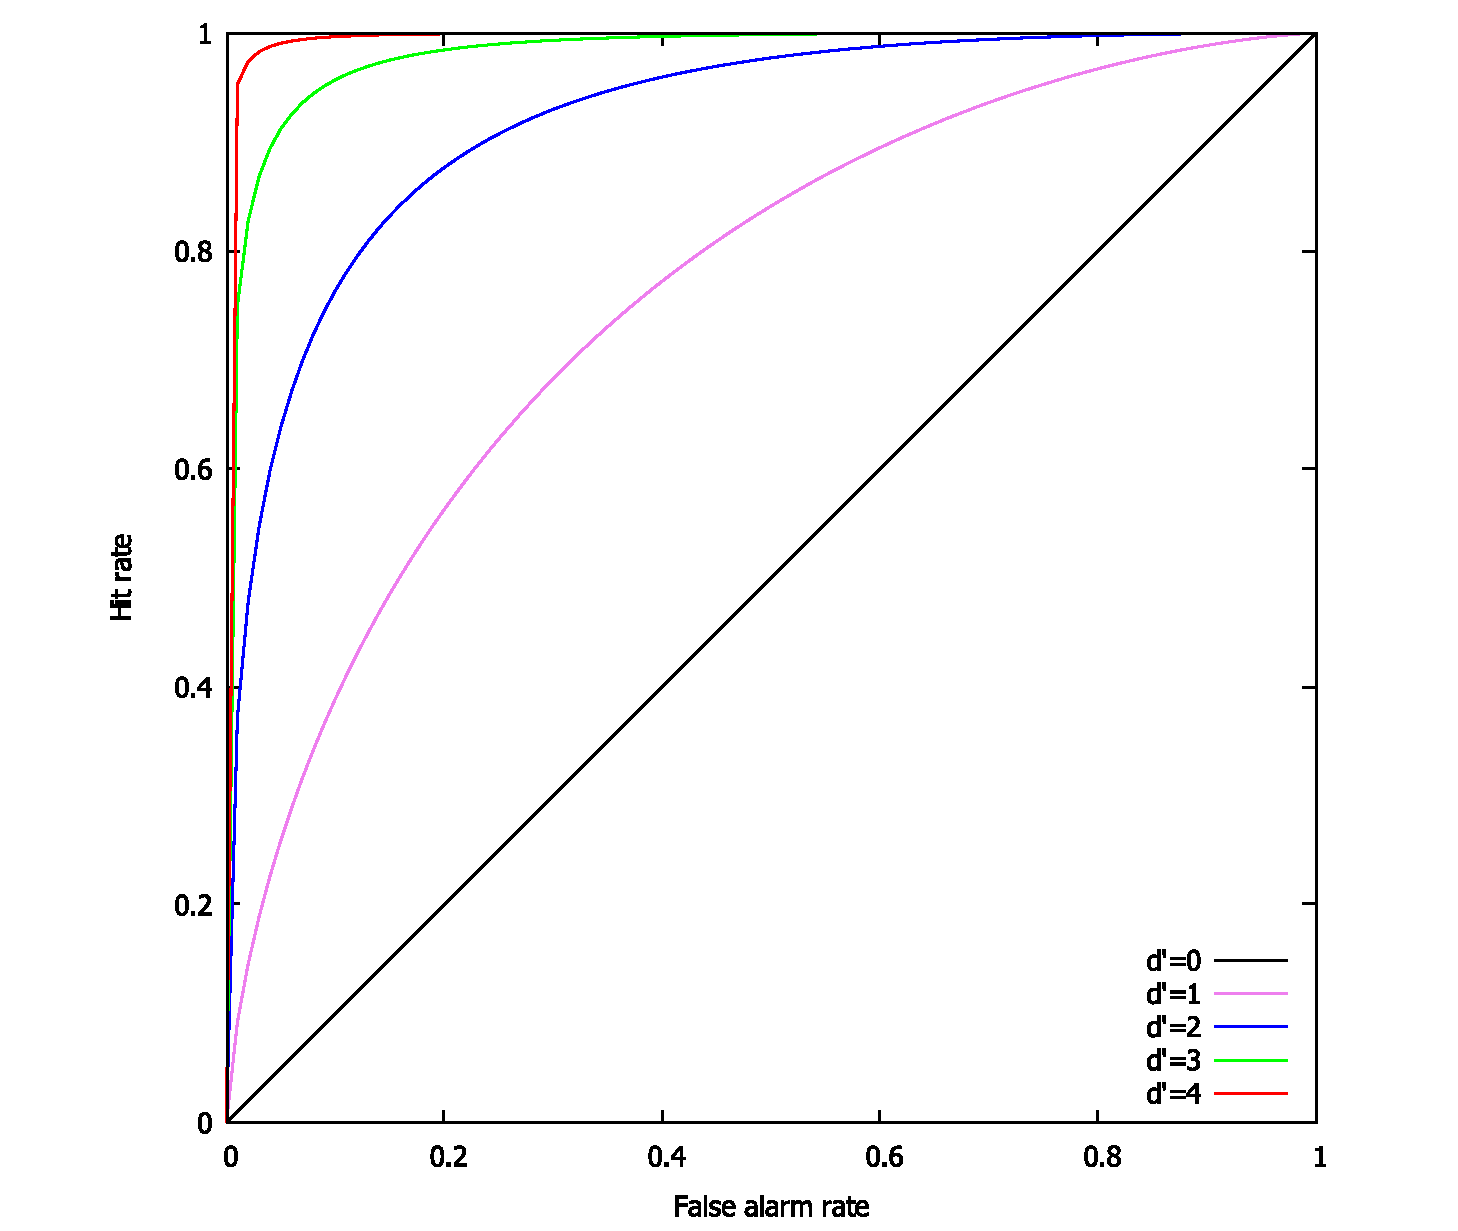
\includegraphics[width=.8\linewidth]{graphs/ROC.pdf}
  \centering
\caption{Závislost hit rate a false alarm rate pro různé hodnoty $d'$. Těmto křivkám se říká ROC křivky z~anglického Receiver Operating Characteristic \citep{SwetsSDT,GreenSDT}.} 
\label{obr:dprime} 
\end{figure}


Nahlédneme, že senzitivita má následující vlastnosti:
\begin{itemize}
\item Pokud $d' = 0$, jsou indikátorové náhodné veličiny \uv{Pozorovatel odpověděl kladně} a \uv{Signál je přítomen} nezávislé.
\item Pokud $d' > 0$, mají tyto dvě veličiny kladnou korelaci.
\item Pokud skutečně má náhodná veličina $X$ jak v~případě, že signál přítomen je, tak v~případě, že signál přítomen není, normální rozdělení lišící se pouze střední hodnotou, pak hodnota $d'$ nezáleží na nastavení kritéria (samozřejmě krom případů, kdy kritérium nastavíme na plus nebo mínus nekonečno, pak hodnota $d'$ není dobře definovaná).
\end{itemize}

Závislost hit rate a false alarm rate pro konkretního pozorovatele se nazývá {\it ROC křivka} z~anglického Receiver Operating Characteristic \citep{SwetsSDT,GreenSDT}. ROC křivky pro vybrané hodnoty $d'$ jsou zobrazeny na obrázku \ref{obr:dprime}.  

\section{Šum}

\index{Šum}
V~teorii detekce signálu šumem nazýváme nechtěnou (a typicky neznámou)
modifikaci signálu.  Signály a s~nimi spojené modifikace mohou být různé
podstaty, například zvukové, nebo se může jednat o~šum v~elektromagnetickém
vlnění. Také se může na signálu projevit mnoha různými způsoby. Může se k~němu
například přičíst. Takový šum nazveme {\it aditivní}. Dále existuje například
 šum multiplikativní či fázový (šum, který se projevuje krátkodobým
fázovým posunem signálu).

Pro úlohu zrakového vyhledávání je relevantní aditivní vizuální šum. Nabízela
by se otázka, proč nepoužít reálnou scénu, nebo naopak jednobarevné pozadí.
Praktické scény jsou však těžko popsatelné a jednobarevné scény (obsahující
pouze diskrétní rozptýlení) vnášejí do formalizace vyhledávání nepřesnosti --
jejich popis je však nad rámec této práce, lze ho najít v~článku
Pelliho a Farella \citeyearpar{WhyNoise}.

  

\subsection{Barva šumu}

I~když však
odhlédneme od média, v~němž se šum šíří či v~něm je zachycený, existuje mnoho
různých šumů. Jeden z~parametrů, který lze měřit, se nazývá {\it výkonová
spektrální hustota}. Její jednotkou jsou watty na Hertz a udává, jaký výkon má šum na dané frekvenci. Máme-li hodnoty šumu v~dostatečně mnoha bodech, jeho spektrální hustotu spočítáme tak, že na šum aplikujeme
Fourierovu transformaci.

V~závislosti na distribuci výkonu napříč různými frekvencemi přiřadíme šumu jméno. Tato jména jsou (i pro jiný než vizuální šum) odvozena od analogie s~viditelným světlem -- šum se pojmenuje podle barvy, jakou by mělo světlo se stejným rozdělením výkonu napříč viditelným spektrem, jaké má šum rozdělení výkonu napříč svým spektrem. Takto známe například bílý, růžový, červený (někdy též označovaný jako
Brownův či nesprávně hnědý\footnote{V anglické literatuře se používá
termín {\it Brownian noise}, setkáme se ale i se zavádějícím
termínem {\it Brown noise}. Jméno je odvozeno od souvislostí s~Brownovým pohybem částic}) či modrý šum (viz obrázek \ref{obr:noise:example}).
\index{Šum!bílý}
\index{Šum!červený}
\index{Šum!růžový}
\index{Šum!modrý}

Spektrální hustotu $p$ všech zmíněných šumů na dané frekvenci $f$ lze vyjádřit jako
$p=1/f^\beta$, kde hodnota $\beta$ je $-1$ pro modrý šum, $0$ pro bílý, $1$ pro
růžový a $2$ pro hnědý. Proto se růžový šum někdy též označuje jako $1/f$ šum. Pro
ostatní barvy šumu není podobné označení běžné. O~šumu a jeho barvách je pojednáno více
v~knize Noise \citep{Noise}.

Pravděpodobnostní rozdělení jednotlivých složek Fourierovy transformace ale
není definicí barvy šumu dáno. Pokud je rozdělení normální (Fourierova obrazu
nebo samotného šumu), řekneme, že se jedná o~gaussovský šum.

V~této práci se budeme zabývat vizuálním šumem, tedy šumem, kde místo obvykle
používané časové souřadnice použijeme dvě souřadnice prostorové a měřenou
hodnotou bude jas. 

\begin{figure}[h!]
\begin{tabular}{cc}
\begin{subfigure}{0.45\textwidth}
  \centering
  
\includegraphics[width=.8\linewidth]{img/blue_noise}
  \caption{Modrý šum} 
\end{subfigure}&
\begin{subfigure}{0.45\textwidth}
  \centering
  
\includegraphics[width=.8\linewidth]{img/white_noise}
  \caption{Bílý šum} 
\end{subfigure}\\
\begin{subfigure}{0.45\textwidth}
  \centering
  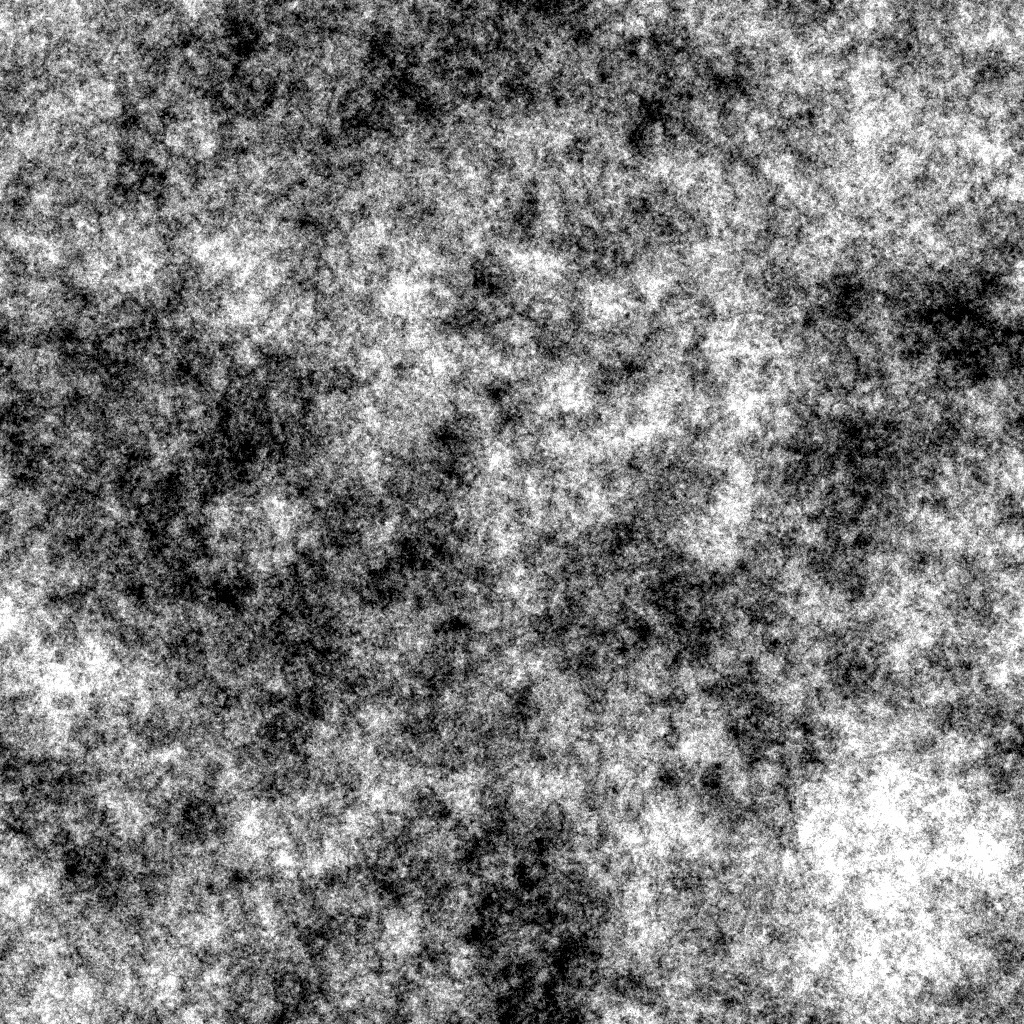
\includegraphics[width=.8\linewidth]{img/pink_noise}
  \caption{Růžový šum} 
\end{subfigure}&
\begin{subfigure}{0.45\textwidth}
  \centering
  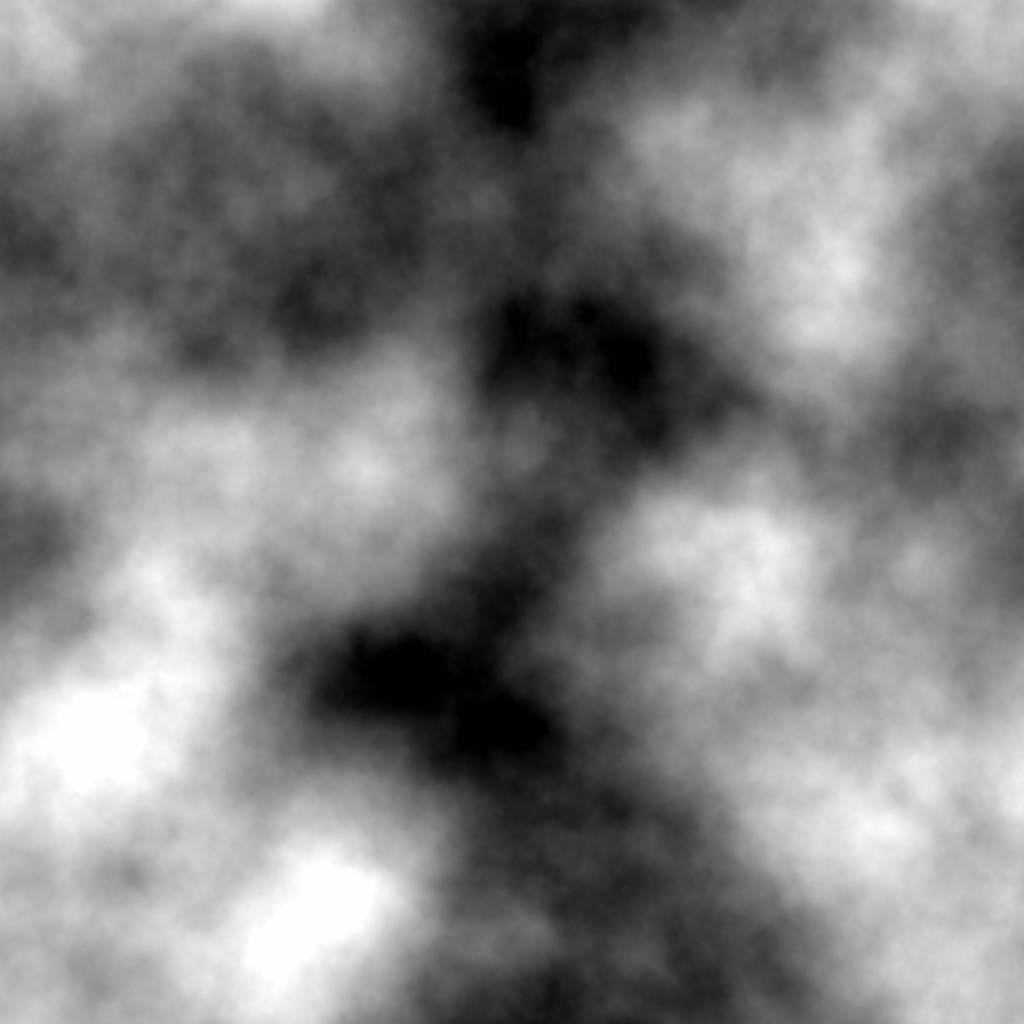
\includegraphics[width=.8\linewidth]{img/brown_noise}
  \caption{Červený, někdy též Brownův šum} 
\end{subfigure}%
\end{tabular} 
\caption{Ukázky různých šumů. Tyto šumy byly vygenerovány pomocí algoritmu použitého přímo v~aplikaci, která je součástí této práce. Algoritmus je blíže popsán ve druhé příloze.} 
\label{obr:noise:example} 
 
\end{figure}
\section{Gabor patch}

\index{Gabor patch}

V~úloze zrakového vyhledávání potřebujeme také nějaký cíl. V~reálném životě
vnímáme mnoho různých podnětů. Pro takovou situaci by však bylo příliš obtížné
najít model. Proto se často používají jednodušší, lépe popsatelné cíle.  Jedním z~takových
stimulů je {\it Gabor patch} vycházející z~Gaborova filtru.

Gaborův filtr (v~českých textech někdy označovaný jako Gaborova vlnka) je
lineární filtr používaný ve zpracování obrazu, chceme-li detekovat signál
mající danou frekvenci a směr, který se vyskytuje kolem daného bodu.

\subsection{Definice}

Hodnotu filtru v~daném bodě spočítáme jako součin dvou funkcí. První z~nich
nazveme {\it jádro} filtru. Jako jádro se vždy používá sinus či cosinus (někdy
uváděné v~podobě komplexní exponenciály, pokud potřebujeme jak reálnou, tak
imaginární složku). Jeho parametry určují, jaké vlastnosti má mít signál, který
chceme detekovat. Druhé funkci říkáme {\it obálka}, a určuje, na jakém okolí daného
bodu signál zkoumáme.

Funkci tedy lze vyjádřit jako $$g(x,y) =
\sin\left(2\pi\frac{x'}{\lambda}+\phi\right)\cdot\operatorname{obálka}(x',y'),$$
kde vektor $(x',y')$ je vektor $(x,y)$ otočený o~úhel, který svírá osa $x$
se směrem, podél nějž chceme měřit signál (tento úhel budeme značit $\Theta$),
a posunutý do bodu, v~němž chceme měřit signál, $\lambda$ je frekvence signálu,
který hledáme, a $\phi$ je fázový posun \citep{GaborPatch}. Frekvence signálu
se nejčastěji udává v~cyklech na jednotku vzdálenosti, často na pixel obrazu.

Jako obálka se používá dvojrozměrná Gaussova funkce, raised cosine, nebo prostá
lineární funkce vzdálenosti. 

Gaussovu funkci vyjádříme jako $$ \operatorname{obálka}(x',y') =
\exp\left(\frac{x'^2 + y'^2}{2\rho}\right),$$ kde $\rho$ je směrodatná odchylka
Gaussovy křivky. Její výhodou je, že chování Gaborova filtru, jehož obálku tvoří
Gaussova funkce, je nejpřesněji popsané. Raised cosine vyjádříme jako 
$$
\operatorname{obálka}(x',y')=
\begin{cases}
 \frac{\cos(\pi\sqrt{x'^2+y'^2}/r)+1}2 &\text{pro $\sqrt{x'^2+y'^2}\leq r$,}\\[1ex]
 0 &\text{jinak,}
\end{cases}
$$ kde $r$ je poloměr oblasti, v~níž chceme signál detekovat. Výhodou raised
cosine oproti Gaussově funkci je, že ve vzdálenosti alespoň $r$ od středu
filtru jeho hodnota nabývá nuly. Při výpočtech tedy stačí počítat s~malou
oblastí kolem středu (kdežto při použití Gaussovy funkce je nutné počítat
s~celým obrazem). Výhodou oproti lineární funkci vzdálenosti je, že raised cosine
se pro většinu aplikací chová dostatečně podobně jako Gaussova funkce.

\subsection{Použití}

Chceme-li detekovat signál ve vizuálním šumu, spočítáme hodnotu $$s=\sum
g(x,y)\cdot n[x,y],$$ kde $n$ je šum, přičemž sumu bereme přes všechny body $(x,y)$,
v~nichž jsme naměřili hodnoty šumu. Je-li hodnota $s$  blízko nuly, signál
v~daném místě není přítomen, nebo je přítomen s~jinými parametry. Vysoké hodnoty
značí, že
signál pravděpodobně přítomen je, hluboce záporné značí, že signál je přítomen,
ovšem s~fází posunutou o~$\pi$.

Gabor filter ale můžeme používat i k~samotné tvorbě signálu. Chceme-li vytvořit
v~daném bodě signál, můžeme spočítat Gabor filter, jako bychom chtěli
detekovat signál s~právě takovými parametry, jaké má mít tvořený signál, a
potom ho sečíst se šumem. Takto vytvořenému signálu budeme říkat Gabor patch (několik příkladů viz obrázek \ref{obr:gabor:example}).

\begin{figure}[h!]
\begin{subfigure}{0.25\textwidth}
  \centering
  
\includegraphics[width=.8\linewidth]{img/gabor1}
\end{subfigure}% 
\begin{subfigure}{0.25\textwidth}
  \centering
  
\includegraphics[width=.8\linewidth]{img/gabor2}
\end{subfigure}% 
\begin{subfigure}{0.25\textwidth}
  \centering
  
\includegraphics[width=.8\linewidth]{img/gabor3}
\end{subfigure}% 
\begin{subfigure}{0.25\textwidth}
  \centering
  
\includegraphics[width=.8\linewidth]{img/gabor4}
\end{subfigure}% 

\caption{Ukázky několika Gabor patchů. Všechny Gabor patche jsou 100 pixelů
široké i vysoké. Levý patch má $\Theta = 1/4\pi$, ostatní mají $\Theta =
-1/4\pi$, levý má jako obálku Gaussovu funkci, prostřední dva raised cosine,
pravý lineární funkci vzdálenosti, první, druhý a čtvrtý patch mají frekvenci
(v~cyklech na pixel) $0.1$, třetí $0.02$.} 

\label{obr:gabor:example} 
 
\end{figure}


\section{Entropie}

\index{Entropie}
\index{Shannonova entropie}
Další pojem, který budeme v~této práci potřebovat, pochází z~teorie informace.
Entropií (nazývanou též Shannonova entropie) náhodné veličiny se v~této teorii
rozumí střední hodnota informace, kterou nám hodnota této veličiny přinese.
Například mějme náhodné veličiny $X$ a $Y$\!. $X$ nechť nabývá hodnoty 0
s~pravděpodobností $1/2$ a hodnoty 1 s~toutéž pravděpodobností. $Y$ nechť nabývá
hodnoty 1 s~pravděpodobností 1 a hodnoty 0 s~pravděpodobností 0. Je vidět, že
pokud se dozvíme, jaké hodnoty nabývá veličina $X$, získáme více informace, než
když zjistíme, jaké hodnoty nabývá $Y$.  \def\H{\operatorname{H}}

Hodnotu informace, kterou nám přineslo zjištění, že náhodná veličina $A$ nabývá
hodnoty $a$, spočítáme jako $$I(A=a)=-\log_b\left({\P{A=a}}\right)=\log_b\left(\frac1{\P{A=a}}\right).$$ Jako
základ logaritmu $b$ se běžně používá 2 (což budeme dodržovat i v~této práci) nebo $e$. 
Všimneme si, že toto vyjádření množství informace je konzistentní
s~intuitivní představou, že pokud $A$ nabývá nějaké nepravděpodobné
hodnoty, je informace o~této hodnotě cennější, než kdyby nabývalo nějaké pravděpodobné. Odsud tedy
entropii $\H(A)$ lze vyjádřit jako $$\H(A)=\mathbb{E}[I(A)]=-\displaystyle\sum_{a
\in \Omega}\P{A=a}\log_2{\P{A=a}},$$ kde $\Omega = \{a\mid\P{A=a} > 0\}$.
Všimneme si, že podle tohoto vzorce je entropie veličiny $X$, tak jak byla
nadefinována v~předchozím odstavci, rovna jedné, kdežto  entropie veličiny $Y$
je rovna nule.

Podobně jako u~pravděpodobnosti můžeme poměrně přímočaře nadefinovat 
i~podmíněnou entropii $\H(A\mid B)$

Shannonova entropie byla v~této podobě zavedena Claudem Shannonem v~jeho článku \citeyearpar{Entropie}. 

\section{Psychofyzika}

Psychofyzika je disciplína psychologie, která zkoumá vztah mezi konkrétními
stimuly a jim odpovídajícími vjemy. Lze ji aplikovat na libovolný smyslový
vjem, ať už obraz, zvuk, vůni, chuť či hmatový vjem \citep{psychophysics}.
Funkcím, které dávají do souvislosti parametry stimulů a chování subjektu
v~experimentu, se říká {\it psychometrické funkce}. 

Při detekci signálu rozeznáváme dva druhy šumu. Šum vnitřní a šum vnější \citep{DavidSDT}.
Vnější šum je zkreslení dat, které nastane ještě mimo pozorovatele. Vnitřní
šum je naopak šum způsobený přímo algoritmem, který používá
pozorovatel, aby dekódoval, zda signál je přítomen, či není.\index{Šum}

Vrátíme se zpět na začátek této kapitoly k~příkladu s~chodcem přecházejícím silnici.
Vnější šum tam může být způsoben množstvím faktorů. Například může nějaký
předmět částečně blokovat výhled. Nebo může být chodcův zrak nedokonalý. Nebo
se může směrem, ze kterého by se mohlo blížit auto, nacházet nějaký jiný předmět, který
vypadá trochu jako auto. Vnitřní šum je naopak čistě uvnitř mozku, kdy mozek
vjem, u~kterého k~tomu nemá žádný důvod, vyhodnotí jako přijíždějící auto.

Právě chování tohoto vnitřního šumu zkoumá psychofyzika.

\section{Modely pozorovatele}

V~teorii detekce signálu je velmi důležitým konceptem ideální detektor.
Mohlo by se nám zdát, že by nás ideální pozorovatel nemusel zajímat -- pracujeme
přece s~pozorovatelem lidským. Pro lidského pozorovatele ale potřebujeme srovnání.
V~případě, kdy je algoritmus ideálního pozorovatele v~určitém smyslu
přirozený, například nedělá žádné kontraintuitivní kroky, můžeme také tvrzení
\uv{Lidský pozorovatel se chová ideálně} použít jako úvodní hypotézu, kterou
poté už pouze upravujeme či zpřesňujeme \citep{GreenSDT}.

\index{Gabor patch}
\index{Šum!růžový}
V~této práci se budeme zabývat úlohou, kdy pozorovatel hledá Gabor patch
v~kruhovém poli, v~němž se nachází růžový šum. 

Abychom mohli hodnotit fixace lidského pozorovatele, potřebujeme mít nějaký
model, který nám bude říkat, jak se chová optimální pozorovatel v~této úloze. Nejprve ale
stručnou odbočku:

\subsection{$d'$ mapa}

\index{d' mapa@$d'$ mapa}
\index{d'@$d'$}
Ještě předtím, než začneme zjišťovat, podle jakého modelu se chová lidský
pozorovatel, je nutné zjistit, kolik informace člověk jednou fixací získá. Je
například zjevné, že kdyby jedním pohledem bez ohledu na to, kam se dívá,
získal stejné množství informace o~všech možných polohách cíle, jsou všechny
modely ekvivalentní. Proto je potřeba najít tzv. $d'$ mapu, funkci, která nám
pro každé dva body $a$, $b$ řekne, jakou hodnotu $d'$ má lidský pozorovatel,
pokud hodnotí pozici $b$ a dívá se na pozici $a$. U~pozadí s~uniformními nebo
téměř uniformními lokálními kontrasty lze tuto funkci zjednodušit, stačí, když
budeme pro každý bod $a$ vědět, jaká je hodnota $d'$ pro rozhodování, zda je
cíl v~bodě $a$, pokud zafixujeme střed.

Jedná se tedy o~psychometrickou funkci, kde je parametrem poloha stimulu, a chování subjektu je vyjádřeno jeho hodnotou
$d'$.

Předchozí výzkum ukázal, že u~běžného člověka je $d'$ mapa poměrně
nepravidelná \citep{Najemnik08}, ale dá se s~přijatelnou přesností aproximovat mapou, kde křivky
spojující body se stejnou hodnotou $d'$ jsou tvořeny čtyřmi čtvrt\-elipsami
(jednou v~každém kvadrantu) se středem v~počátku,
s~excentricitami a velikostí poloos danou hodnotou $d'$ a individuálními
vlastnostmi pozorovatele a cíle \citep{Ellipse}. 

Ke kompletnímu vyjádření aproximace funkce $d'$ potřebujeme celkem 6 hodnot,
které závisí na konkrétním pozorovateli a cíli. Jedná se o~hodnotu $d'_0 =
d'(0,0)$, hodnot $e_L$, $e_R$, $e_U$ a $e_D$, které určují vzdálenost ve čtyřech
základních směrech takovou, že v~nich je hodnota $d'$ poloviční oproti počátku,
a hodnotu $\beta$ popisující sklon této funkce. Funkci $d'$ pak vyjádříme jako
$$ d'(x,y) = \frac{d'_0}{1+\left(\frac{x^2}{e_H^2}+\frac{y^2}{e_V^2}
\right)^\beta}, $$ kde $e_H$ je rovno $e_L$ pro záporná $x$ a $e_R$ pro kladná,
a $e_V$ je rovno $e_D$ pro záporná $y$ a $e_N$ pro kladná.


\subsection{Modely chování pozorovatele}

Všechny modely, které zde budeme zkoumat, vypadají tak, že mají tzv. {\it mapu
aposteriorních pravděpodobností}. V~této mapě je pro každou lokaci, kde by
signál (též cíl) mohl být, uvedeno, jaká je pravděpodobnost, že se na ní cíl
nachází, vzhledem k~informaci, kterou již o~dané lokaci pozorovatel získal. 

Pozorovatel postupuje tak, že si vždy vybere lokaci, kterou zafixuje. Poté
provede fixaci a získá o~každé lokaci určitou informaci. Pak spočítá novou mapu
aposteriorních pravděpodobností. Pokud na některé lokaci pravděpodobnost přesáhne kritérium, pozorovatel
ukončí hledání a ohlásí nalezení cíle na této lokaci. Jinak pokračuje ve vyhledávání výběrem další lokace k~fixaci.
Jednotlivé modely se dále liší pouze algoritmem, který používají k~výběru lokace k~fixaci.


V~rámci předchozího výzkumu bylo otestováno mnoho modelů, jako například
pozorovatel, který volí fixace náhodně, nebo pozorovatel, který volí fixace 
tak, aby nikdy nezafixoval tutéž lokaci vícekrát. Všechny tyto modely se ale ukázaly jako
nevhodné vzhledem k~tomu, že v~praxi dosahují mnohem horších výsledků (měřeno
pomocí střední hodnoty počtu fixací před nalezením cíle) než lidský
pozorovatel \citep{Najemnik05}.

\subsubsection{MAP pozorovatel}

\index{MAP pozorovatel}
Nejjednodušší model, který dosahuje podobných výsledků jako lidský pozorovatel,
je tzv. MAP pozorovatel (zkratka je odvozena z~anglického \uv{Maximum Aposteriori Probability}),
 který vždy zafixuje lokaci, která má v~jeho mapě aposteriorních
pravděpodobností nejvyšší hodnotu. Tento pozorovatel již dosahuje podobných
výsledků jako lidský, ale jeho strategie fixací neodpovídá strategii, jakou
volí lidský pozorovatel. Lidský pozorovatel umístí svoji první fixaci do středu
scény. Ostatní fixace jsou pak rozmístěny v~okolí kružnice se středem ve středu
scény a poloměrem rovným přibližně $2/3$ poloměru scény, s~preferencí pro horní
a spodní okraj. MAP pozorovatel oproti tomu vybírá každou lokaci se zhruba
stejnou pravděpodobností.

\subsubsection{Ideální Bayesovský pozorovatel}

\index{Ideální Bayesovský pozorovatel}
\index{IBO}
Ještě o~trochu lepších a hlavě statisticky lidskému pozorovateli bližších
výsledků dosahuje model Ideálního Bayesovského pozorovatele.  

Ideální Bayesovský pozorovatel (dále IBO) je pozorovatel, který poté, co již provedl $T$ fixací, vybírá následující lokaci
tak, aby maximalizoval pravděpodobnost, že v~následujícím kroku odhalí
cíl. Vybere tedy lokaci 
\begin{equation}\label{IBOnext}k_{opt}(T+1) = \displaystyle{\operatorname{arg\ 
max}}_{k(T+1)} \left(\displaystyle\sum_{i\in L} p_T(i)\P{p_{T+1}(i)\geq c\mid i,
k(T+1)}\right),
\end{equation} 
kde $p_N$ je mapa aposteriorních pravděpodobností po $N$-té
fixaci, $L$ je množina všech potenciálních lokací cíle a $c$ je kritérium,
které musí hodnota v~mapě aposteriorních pravděpodobností překročit, aby bylo
ukončeno hledání a nahlášeno nalezení cíle. Výraz $\P{p_{T+1}(i)\geq c \mid
i,k(T+1)}$ pak tedy znamená \uv{pravděpodobnost, že po $(T+1)$-ní fixaci bude
ukončeno hledání a nahlášen signál v~lokaci $i$, za podmínky, že v~ní signál
opravdu je přítomen a byl zafixován bod $k(T+1)$}. 

IBO však ale též není příliš dobrým kandidátem na model, podle nějž se
lidé chovají.  Ač má jeho vyhledávání podobné statistické vlastnosti jako
vyhledávání lidského pozorovatele, vyžaduje perfektní paměť a ideální integraci
informace mezi fixacemi. Ani jednu z~těchto dovedností ale lidský pozorovatel
nemá. Dále si můžeme všimnout, že přinejmenším přímočaré
vyhodnocení výrazu \eqref{IBOnext} je kubické v~počtu potenciálních
lokací (výpočet druhého činitele součinu v~sumě je lineární, suma sama je přes
lineárně mnoho členů a vnější maximum má též lineárně mnoho možných voleb
$k(T+1)$). Lidský pozorovatel při vyhledávání volí další fixaci přibližně
třikrát až čtyřikrát za vteřinu, je tedy nepravděpodobné, že by lidský mozek
dokázal takový výpočet provést \citep{Najemnik08}. 

\subsubsection{ELM pozorovatel}

\index{ELM pozorovatel}
\index{Entropie}
ELM (z~anglického \uv{Entropy limit minimization}) pozorovatel je
pozorovatel, který při výběru následující fixace minimalizuje střední hodnotu
entropie náhodné veličiny určující lokaci cíle po fixaci. Tu spočítáme jako
\begin{equation}\label{EntropyBasic}\E{\H(T+1)\mid k(T+1)}=-\E{\displaystyle\sum_{i\in
L}p_{T+1}(i)\log_2p_{T+1}(i)\mid k(T+1)}.\end{equation} \citet{Najemnik09} však ukázali,
že vyjádření hodnoty entropie podle vzorce \eqref{EntropyBasic} je sice
netriviální, ale lze ho dobře aproximovat případem, kdy pošleme v~limitě $|L|$
do nekonečna. Pak dostáváme výraz $$ \E{\H(T+1)\mid k(T+1)}= \H(T) -
\displaystyle\sum_{i\in L} p_T(i)d'^2(i-k(T+1)),$$ kde v~posledním členu bereme
lokace jako vektory od počátku k~nim. Člen $\H(T)$ navíc nezávisí na $k(T+1)$,
takže s~ním vůbec nemusíme počítat a k~minimalizaci entropie nám stačí
maximalizovat hodnotu sumy.


\section{Percepční učení}
\index{Percepční učení}

Při opakovaném vykonávání téže úlohy týmž člověkem dochází k~postupnému
zlepšování výkonu. Jedná-li se o~úlohu související se smyslovým vnímáním, je
jedním z~faktorů vedoucích ke zlepšení percepční učení. To znamená, že se samy
smyslové orgány a části mozku určené ke zpracování vjemů z~těchto orgánů
zlepšují v~rozpoznávání daných stimulů. Toto zlepšení je relativně dlouhodobé,
i bez opakování vydrží smyslovému orgánu zvýšená citlivost na daný typ stimulu
řádově měsíce \citep{uceni2}.

Percepční učení se týká všech pěti smyslů. Přestože se o~něm nejčastěji mluví
ve spojení se zrakem či sluchem, existují výzkumy, při kterých byla například v~mozku
houslistů naměřena silnější odezva při lehkém doteku špiček jejich prstů na levé ruce oproti ruce pravé \citep{violinists}. To je konzistentní s~pozorováním,
že houslisté potřebují jemnější cit v~prstech levé ruky oproti pravé ruce.

Percepčním učením může člověk dosáhnout překvapivých kvalit. Účastníci
experimentu, ve kterém bylo cílem rozhodnout, zda je jedna vodorovná čára
posunutá vůči druhé ve svislém směru nahoru či dolů, byli schopni po dostatečně
dlouhém tréninku dosáhnout přesnosti lepší, než jaká by odpovídala rozlišení
sítnice. Je tomu tak proto, že zorné plochy jednotlivých fotoreceptorů se do
určité míry překrývají, a mozek se naučil vyhodnocovat signály z~fotoreceptorů,
které byly vjemem úsečky zasaženy jen částečně. Jednalo se ale skutečně
o~nízkoúrovňový proces.  V~experimentu, kde účastníci trénovali pouze jedním okem
a poté měli ukázat rozpoznávací schopnost oka druhého, se ukázalo, že se
rozlišovací schopnost přenesla pouze částečně \citep{VisualLinesEye}. V~experimentu, kdy účastníci
používali obě oči se ukázalo, že zlepšení ve vnímání této situace nemá žádný
vliv na schopnost řešit tutéž úlohu otočenou o~devadesát stupňů \citep{VisualLines}.  
Limitace spočívající ve špatném přenosu naučené schopnosti na jiný podobný úkol
je pro percepční učení typická.

Percepční učení není zdaleka jen lidskou schopností. Různé projevy percepčního
učení byly pozorovány například u~mnoha různých druhů savců či ptáků. 

Na rozdíl od ostatních druhů učení, například kognitivního, probíhá percepční
učení zcela podvědomě. Naučenou schopnost nelze vědomě používat či nepoužívat.
\citet{DistraktoryCile} provedli sadu experimentů, kdy v každé sadě měli
účastníci co nejrychleji reagovat na dané písmeno. Lidé, kteří dostávali v
každé sadě stále nová a nová písmena, dopadali lépe, než lidé, kteří měli jako
distraktor písmeno, na které měli v předchozích testech reagovat. Další výzkum
\citep{ANaopak} ukázal, že lidé reagují pomaleji na písmeno, které pro ně v
předchozích testech sloužilo jako distraktor, než na písmeno, které v
experimentu dříve neviděli. Percepční učení nevyužívá deklarativní paměť, což
znamená, že člověk, který si prostředky percepčního učení osvojil nějakou
schopnost, nedokáže říci, co dělá jinak, než před učením. Probíhá i zcela bez
zpětné vazby. V~jednom experimentu se například měly myši naučit rozeznávat
různé symboly. Některé z~nich však měly tyto symboly již před experimentem
umístěné na místě viditelném z~klece. Tyto myši pak dosáhly v~testu rychlosti
učení lepších výsledků, než myši, které symboly nikdy dříve neviděly
\citep{Rats}. Odměna za splnění úkolu však percepční učení urychluje.

Percepční učení probíhá celkem čtyřmi způsoby. O~těch je blíže pojednáno
v~článku \citep{uceni}, my je zde pouze stručně představíme. Pro jejich popis použijeme původní anglickou terminologii. Jedná se o:

\begin{itemize}
\item Attentional weighting -- Člověk se učí rozlišovat aspekty stimulu,
které jsou důležité. Například v~experimentu, kde má člověk odlišit červená
písmena od modrých, začne brzy věnovat tvaru písmene menší pozornost, aby se
mohl lépe soustředit na barvu.
\item Stimulus imprinting -- Samotné koncové smyslové orgány se vyvíjí, aby
lépe rozpoznaly stimul nebo některé jeho části.
\item Differentiation -- Lidé se učí rozeznávat nejen hodnoty atributů stimulu,
které by pro ně dříve byly nerozlišitelné (viz příklad s~vodorovnými přímkami výše), ale i zcela nové atributy stimulů (například když se rodiče učí rozpoznávat od sebe svá dvojčata, rozeznávají je podle vlastností, jejichž rozdílnosti si dříve u~lidí obecně nebyli vědomi).
\item Unitization -- Lidé si z~bloků vytvořených předchozím způsobem, určených k~rozeznávání jednotlivých aspektů stimulů, staví komplikovanější struktury rozpoznávající celé stimuly. 
\end{itemize}

Mohlo by se zdát, že poslední dva principy jdou proti sobě. První z~nich se
však používá v~případě, kdy je nutné rozpoznávat mnoho různých druhů stimulů
(například rozeznávání mnoha různých ne příliš blízkých lidí), druhý z~nich
v~případě, že se některé vlastnosti stimulů často vyskytují současně a jsou tedy
svým způsobem redundantní. Hodí se při rozpoznávání písmen v~psaném, či celých
slov v~psaném i mluveném projevu.
